\section{Maciej Michałek}
\label{sec:macmichalek}

Tutaj wstawiam przykładowe wyrażenie.
\begin{equation}
    \sum_{k=1}^{2n} k
    \label{fig:wyrazeniemat}
\end{equation}

\vspace{2em}
Dodałem poniżej zdjęcie słodkiej pandy (zobacz Rysunek ~\ref{fig:funnypanda}).

\begin{figure}[htbp]
    \centering
    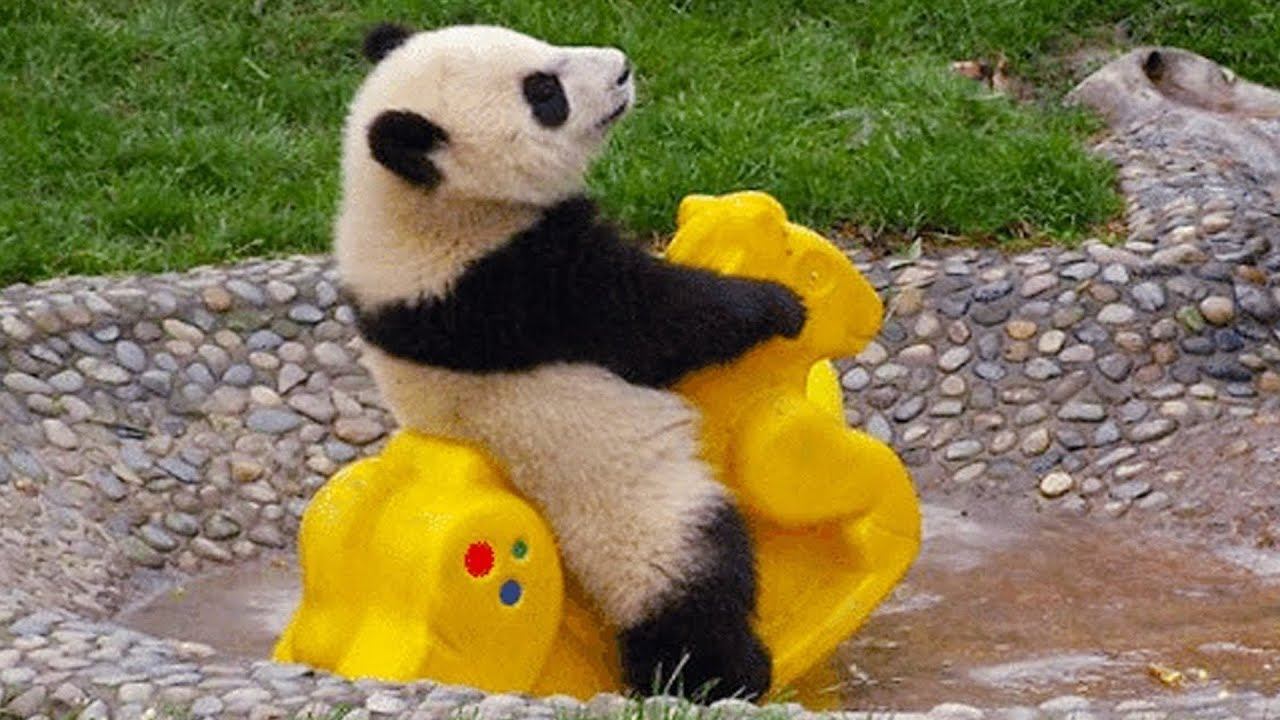
\includegraphics[width=0.5\textwidth]{pictures/funny panda.jpg} 
    \caption{"I love this konik."}
    \label{fig:funnypanda}
\end{figure}

\vspace{2em}
Randomowa tabelka.

\begin{table}[h]
\begin{tabular}{|c|c|c|ll}
\cline{1-3}
\cellcolor[HTML]{6200C9}Literki & \cellcolor[HTML]{6200C9}Cyferki & \cellcolor[HTML]{6200C9}Znaczki &  &  \\ \cline{1-3}
A & 1 & !  &  &  \\
B & 2 & @  &  &  \\
C & 3 & \# &  &  \\ \cline{1-3}
\end{tabular}
\centering
\label{tab:mmichalek_tab}
\caption{Prosta tabelka taka o.}
\end{table}

\vspace{2em}
Tutaj wrzucę kilka numerków:
\begin{enumerate}
  \item I cyk jedyneczka
  \item Kolejna dwujeczka 
  \item Last one to trójeczka
\end{enumerate}

\vspace{1em}
Tutaj kolejne punkciki:
\begin{itemize}
  \item Zwykła kropeczka
  \item[!] Tutaj coś ciekawszego
  \item[>] A tu strzała
\end{itemize}

\section*{Opis pandy z wiki}
{\bf Panda wielka} - niedźwiedź bambusowy {\it (Ailuropoda melanoleuca)} – gatunek drapieżnego ssaka z rodziny niedźwiedziowatych (Ursidae).
\section*{Opis cd}
{\bf Panda wielka} zamieszkuje lasy bambusowe na wysokości 1200–4100 m n.p.m. (zimą schodzi do 800 m n.p.m.). Jej przynależność do drapieżnych nie ulega wątpliwości, jednak w rzeczywistości odżywia się pędami roślin (głównie bambusa), nie gardzi też rybami i małymi gryzoniami. Zaliczenie pandy do zwierząt drapieżnych spowodowane jest budową jej układu pokarmowego.

\vspace{2em}
koniec.